\documentclass[a4paper]{jsarticle}
\usepackage[dvipdfmx]{graphicx} % Required for inserting images
\usepackage{amsmath}
\usepackage{amsthm}
\usepackage{amssymb}
\usepackage[margin=20truemm]{geometry}
\usepackage{graphicx}
\usepackage{enumerate}
\usepackage{tikz-cd}
\usepackage{tikz}
\usetikzlibrary{intersections,calc,arrows.meta}

 \theoremstyle{definition}
    \newtheorem{dfn}{定義}[section]
    \newtheorem{prop}[dfn]{命題}
    \newtheorem{lem}[dfn]{補題}
    \newtheorem{thm}[dfn]{定理}
    \newtheorem{cor}[dfn]{系}
    \newtheorem{exam}[dfn]{例}
    \newtheorem{rem}[dfn]{注意}
    \newtheorem{hsk}[dfn]{補足}
    \renewcommand\proofname{\bf 証明}

    \renewcommand{\qedsymbol}{$\blacksquare$}
\newcommand{\SimpComp}{{\mathrm{SimpComp}}}
\newcommand{\Fun}[2]{[#1,~#2]}
\newcommand{\Vect}{{\mathrm{Vect}}}
\newcommand{\SimpCompInc}{{\mathrm{SimpCompInc}}}
\newcommand{\grmodZ}{{\mathrm{grmod \mathbb{Z}_2[x]}}}
\newcommand{\Hom}{{\mathrm{Hom}}}
\newcommand{\ob}{{\mathrm{ob}}}
\newcommand{\Ker}{{\mathrm{Ker}}}
\newcommand{\Image}{{\mathrm{Im}}}

\title{graduate book}
\author{猪原 盛寿}
\date{October 19th 2023}


\begin{document}
\Large
\maketitle
「希望を持ちつつ旅をするのは、そこに行き着くことよりも楽しい」\\
---ロバート・ルイス・ スティーブンソン
\section{導入 Introduction}
本稿はパーシステントホモロジーの代数的解釈について, 暗黙的に用いられている同値関係を圏論によって明示し, より広い応用を支える基礎理論への貢献を試みる. \\

パーシステントホモロジーは位相的データ解析の基本的なツールの一つで, 近年著しい発展を遂げており, その応用範囲はDNAの3次元構造から株式市場に至るまで多岐にわたる. 位相的データ解析では, データ$\Rightarrow$空間$\Rightarrow$代数$\Rightarrow$特徴量という順序で, データから位相・幾何的な構造を抽出した値(特徴量)を算出する[1]. パーシステントホモロジーもこれに習うが, 代数の部分を見る際, 次数付き加群としての解釈とベクトル空間としての解釈の二つが存在する. しばしばこの二つは同値として用いられるが, あくまで暗黙的な了解となっている. そこで本稿では次に紹介する圏論を介して明文化することを試みる. \\

直感的なアイデアを他者と共有するには, そのアイデアの形式化を要求される. 概念の形式化とはすなわち数学の仕事であり, 圏論もこれを担う. 数学の中でも特に抽象度の高い圏論では, あらゆる数学的対象を定めた形に書き直すことで, 大域的な関係性を明示する. 例えば, 幾何と代数のような異なる分野の数学的対象の橋渡しも行うことも可能である. \\

本稿の構成は以下の通り. 第2章, パーシステントホモロジーの代数的解釈と圏論の基本的な三つの道具を紹介する. 第3章, パーシステントホモロジーを圏論の観点から記述する. 
\section{背景 background}
パーシステントホモロジーの代数的な解釈のために必要な定義を次に記す. 始めは抽象単体複体である. これはデータ$\Rightarrow$空間と変換するためのツールである. 
\begin{dfn}
    抽象単体複体($V,K$)とは, 以下の条件を満たす数学的構造である.\\
    有限集合$V$と$V$の部分集合の有限個の集まり$K$の組, から構成され次の二つの条件を満たす.\\
    \noindent
    (1)$\; \forall v\in V$ならば, $\{v\}\in K$ \\
    (2)$\; \forall a\in K,$かつ $b\subset a$ならば, $b\in K$
\end{dfn}

\begin{exam}
    $V=\{ \{1\}, \{1,2\}\}, K=\{\{1\}, \{2\}, \{1,2\} \}$とするとき, ($V,K$)は抽象単体複体の定義を満たす. (証明) (1)について, $\{1\}, \{1,2\}\in K$より満たされる. (2)について, $\{1\}, \{2\}\in K$より満たされる. 以上より($V,K$)は抽象単体複体といえる. また$K=\{\{1\}, \{1,2\} \}$とするとき, ($V,K$)は(2)を満たさないため抽象単体複体とはいえない.
\end{exam}
\begin{hsk}
    ここで$\sigma=\{v_0,...,v_k\}\in K$を$k$単体と呼び, その次元を$k$で定める. また$K$に含まれる単体の最大次元を, 抽象単体複体($V,K$)の次元と呼び, dim($V,K$)で定める. 上の例では, $\{1\}, \{2\}$を0単体, $\{1,2\}$を1単体と呼び, dim($V,K$)$=1$である.\\
\end{hsk}
抽象単体複体どうしをつなぐ特別な写像の一つに単体写像がある. これは抽象単体複体の構造を保ったまま単体を写す写像である.
\begin{dfn}
    $(V, K), (V', K')$を抽象単体複体とする. 単体写像$f:K\rightarrow K'$とは, 以下の条件を満たす写像である. $K$の各頂点を$K'$のある頂点に写し次の条件を満たす. 
\begin{equation}
    \forall \{a_0,...,a_q\}\in K\Rightarrow \{f(a_0),...,f(a_q)\}\in K'
\end{equation}
\end{dfn}
\begin{exam}
    $K=\{ \{a\}, \{b\}, \{a,b\}\}, K'=\{ \{x\},\{y\}, \{z\}, \{x,y\}\}$とし, $f:K\rightarrow K'$は$K$の各要素を$f(\{a\})=\{x\}, f(\{b\})=\{y\}$と写すとき, $f$は単体写像の定義を満たす. (証明) $\{f(\{a\}), f(\{b\})\}=\{x,y\}\in K'$より条件を満たすため. また, $f(\{a\})=\{x\}, f(\{b\})=\{z\}$のとき, $f$は単体写像の定義を満たさない.
\end{exam}
\begin{hsk}
    単体写像は単体を写すのではなく頂点のみを写すことに注意したい. 仮に単体そのものを写す写像を単体写像'とすると, 抽象単体複体の構造を保つことなくその写像は機能を失ってしまう. また, 単体の次元の順序関係を保つ条件として, $\sigma\subseteq\tau \Rightarrow f(\sigma) \subseteq f(\tau)$を加えても次元の順序関係のみが保たれ, 単体としては遥か上の次元へと写すことが可能となってしまう. 結果的に, 抽象単体複体の構造をうまく保つ写像を作ろうとすれば, 上記のように頂点のみを写し条件に単体としての構造が保存されることを加えた定義になるのである.\\
\end{hsk}

抽象単体複体によってデータ$\Rightarrow$空間と変換が可能になったが, 次はこの変換によって特徴量が変化しないことを証明する必要がある. その役割を果たすのが脈体定理である.
 
\begin{thm}
    (脈体定理) $X\subset \mathbb{R}^N$が凸閉集合の有限個の集まり$\Phi=\{B_i\subset \mathbb{R}^N| i=1,...,m\}$に被覆されているとする. このとき, 以下の条件を満たす脈体$\mathcal{N}(\Phi)$は, $X$とホモトピー同値となる. 頂点集合を$V=\{1,...,m\}$, 単体の集まり$K$を, 
\begin{equation}
   K = \left\{ \{1,...,k\} \middle| \; \bigcap_{i=1}^{k}B_{i} \neq \emptyset \right\} 
 \notag
 \end{equation}
とすると($\emptyset$ は空集合の意), ($V,K$)は抽象単体複体となる. この抽象単体複体を$\Phi$の脈体と呼び, $\mathcal{N}(\Phi)$で表す.
\end{thm}

\begin{exam}下図は$B_i$を円とするときの脈体の例. 真ん中の穴の情報が保存されていることが分かる.
\end{exam}
\begin{equation}
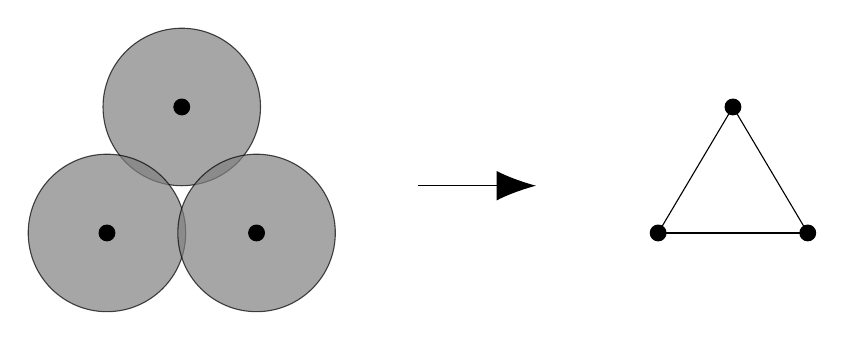
\begin{tikzpicture}
%三つの円%
\filldraw[fill=gray, draw=black, opacity=0.7] (-4,0) circle (1);
\filldraw[fill=gray, draw=black, opacity=0.7] (-4.95,-1.6) circle (1);
\filldraw[fill=gray, draw=black, opacity=0.7] (-3.05,-1.6) circle (1);
%中心点%
\filldraw[fill=black, draw=black] (-4,0) circle (0.1);
\filldraw[fill=black, draw=black] (-4.95,-1.6) circle (0.1);
\filldraw[fill=black, draw=black] (-3.05,-1.6) circle (0.1);
%矢印%
\draw [-{Latex[length=5mm]}]  (-1,-1) -- (0.5,-1);
%三角形%
\filldraw[fill=black, draw=black] (3,0) circle (0.1);
\filldraw[fill=black, draw=black] (3.95,-1.6) circle (0.1);
\filldraw[fill=black, draw=black] (2.05,-1.6) circle (0.1);
\draw (3.95, -1.6) -- (2.05, -1.6);
\draw (3.95, -1.6) -- (3, 0);
\draw (3, 0) -- (2.05, -1.6);
\end{tikzpicture}
\notag    
\end{equation}

\begin{hsk}
$\mathbb{R}^N$は$n$次元ユークリッド空間のこと. 上の図では0単体を頂点, 1単体を頂点を結ぶ線分として表現している. 脈体定理の証明は[参考文献]を参照されたい. \\    
\end{hsk}

次にホモロジー群を定義する. これは空間$\Rightarrow$代数と変換するためのツールである. \\
($V,K$)を$n$次元抽象単体複体とし, それに属する$k$単体すべての集まりを
\begin{equation}
    K_k=\{\sigma_1,...,\sigma_m\in K | \; \dim\sigma_i=k \}\notag
\end{equation}
で表す. $m$は$K$内の$k$単体の個数のことである.自由$\mathbb{Z}$加群とは, 

各次元ごとに$K_k$から生成される自由$\mathbb{Z}$加群$C_k(K)$を次のように定義する.
\begin{equation}
   C_k(K)= \mathbb{Z}\langle K_k\rangle = \left\{ c=\sum_{i=1}^{m}\alpha_i\sigma_i \middle| \; \alpha_i\in\mathbb{Z} \right\} 
 \notag
\end{equation}
$k<0, n<k$のとき, $C_k(K)=0$とする. これにより, 抽象単体複体を代数的に表現することができる. 次に$C_k(K)$の各次元をつなぐ写像を定義する. これは不変量を計算するホモロジー群を生成するために必要となる. この写像は境界作用素と呼ばれる. 各$0\leq k\leq n$に対して, 境界作用素$\partial_k:C_k(K)\rightarrow C_{k-1}(K)$は$C_k(K)$の任意の単体$\sigma_i=\{v_0,...,v_k\}$を次のように写すものである. 
\begin{equation}
    \partial_k(\sigma_i)=\sum_{j=0}^{k} (-1)^j \{v_0,...,\hat{v_j},...v_k\}\notag
\end{equation}
$\{v_0,...,\hat{v_j},...v_k\}$は, $k$単体$\{v_0,...,v_k\}$から$j$番目の$v_j$を除いた$k-1$単体のことである. 例えば, $k=2, \sigma_i=\{v_0,v_1,v_2\}$のとき$\partial_2(\sigma_i)=\{v_1,v_2\}-\{v_0,v_2\}+\{v_0,v_1\}$となる. さらに$\partial_k$は$C_k(K)$の任意の元$c=\sum_{i=1}^{m}\alpha_i\sigma_i$については線形拡張 
\begin{equation}
    \partial_k(c)=\sum_{i=1}^{m}\alpha_if_k(\sigma_i)\notag
\end{equation}
で定義する. また境界作用素は次の重要な性質を満たす. 
\begin{prop}
    すべての$k\in\mathbb{N}$について$\partial_{k-1}\circ \partial_k=0$が成り立つ. 
\end{prop}
(証明) $\sigma_i=\{v_0,...,v_k\}$とすると, 
\begin{equation}
    \begin{array}{lll}
       \partial_{k-1}\circ \partial_k(\sigma_i)  & = & \partial_{k-1}(\sum\limits_{j=0}^{k} (-1)^j \{v_0,...,\hat{v_j},...v_k\})\\
         & = & \sum\limits_{j=0}^{k} (-1)^j \partial_{k-1}(\{v_0,...,\hat{v_j},...v_k\})\\
         & = & \sum\limits_{j=0}^{k} (-1)^j (\sum\limits_{l<j}^{} (-1)^l\{v_0,...,\hat{v_l},...,\hat{v_j},...v_k\}\\
         & & +\sum\limits_{l>j}^{} (-1)^{l-1}\{v_0,...,\hat{v_j},...,\hat{v_l},...v_k\})\\
         & = & \sum\limits_{l<j}^{} (-1)^{i+l}\{v_0,...,\hat{v_l},...,\hat{v_j},...v_k\}\\
         & & +\sum\limits_{l>j}^{} (-1)^{i+l-1}\{v_0,...,\hat{v_j},...,\hat{v_l},...v_k\}\\
         & = & 0 \notag
    \end{array}
\end{equation} 

以上で境界作用素を導入することができた. ここからはホモロジーを定義していきたい.
抽象単体複体$(V, K)$を代数化したものを境界作用素でつないだ系列, 
\begin{equation}
    0\rightarrow C_k(K)\xrightarrow[]{\partial_k} C_{k-1}(K)\xrightarrow[]{\partial_{k-1}}\cdot\cdot\cdot\xrightarrow[]{f_2} C_1(K)\xrightarrow[]{\partial_1} C_0(K)\rightarrow 0\notag
\end{equation}
から, ホモロジーを定義する. \\
部分加群とは, 
次に, $C_k(K)$内の二つの部分加群$Z_k(K), B_k(K)$に着目する. \\
\begin{equation}
    \begin{array}{lll}
       Z_k(K)  & = & \Ker \partial_k =\{c \in C_k(K)| \partial_k(c)=0\}\\
       B_k(K)  & = & \Image \partial_{k+1} = \{c \in C_k(K)| c= \partial_{k+1}(c'), c'\in C_{k+1}(K)\}\notag
       
    \end{array}
\end{equation}
前の命題から$B_k(K)\subset Z_k(K)$が成り立ち, 次のホモロジー群が定義される. 
\begin{dfn}
    抽象単体複体$K$のホモロジー群とは, 剰余加群
    \begin{equation}
        H_k(K)=Z_k(K)/B_k(K)\notag
    \end{equation}
のことである.
\end{dfn}
\begin{dfn}
    次数付き$\mathbb{Z}_2[x]$加群$M$とは, $\mathbb{Z}_2[x]$加群である$M$にアーベル群としての直和分解を与え, $x^jM_i\subset M_{i+j}$を満たすものである($i,j\in\mathbb{N}_0$).
    \begin{equation}
        M=\bigoplus_{i=0}^{\infty} M_i\notag
    \end{equation}
\end{dfn}
\begin{dfn}
    次数付き$\mathbb{Z}_2[x]$準同型写像とは, $M, N$を次数付き$\mathbb{Z}_2[x]$加群とすると, $f:M\rightarrow N$が$\mathbb{Z}_2[x]$準同型写像であって, $f(M_i)\subset N_i$を満たすものである.
\end{dfn}
\begin{dfn}
    $\mathbb{Z}_2[x]$準同型写像とは, $M, N$を$\mathbb{Z}_2[x]$加群とすると, $f:M\rightarrow N$が次の条件を満たすものである. $(a, b\in M)$
        \begin{flalign}
             &(1) f(a+b) = f(a)+f(b)&\\
             &(2) f(xa)= xf(a)& \notag
        \end{flalign}
\end{dfn}
剰余加群とは, 





\noindent\\

自由$\mathbb{Z}$加群, 部分加群\\
剰余加群\\
忠実充満\\
数学には, 「関係性」に着目した極めて抽象的な分野が存在する. それは圏論である. 本稿では圏論の基本的な三つの道具(圏, 関手, 自然変換)を定義し, 第3章へとつなげたい. 手始めに, 圏(category)の定義を確認する.
\begin{dfn}
圏$X$とは以下の条件を満たす数学的構造である. 
\begin{itemize}
    \item 対象(object)の集まり ob($X$)
    \item 射(morphism)の集まり Hom($A,B$)
    (各対象$A, B$に対して$A$から$B$への射の集まりをHom($A, B$)とする)
    \item 射の合成と呼ばれる関数$(\circ)$
\end{itemize}
\begin{equation}
    \begin{array}{lllll}
     \circ &: \Hom (B, C) &\times \Hom (A, B) &\rightarrow &\Hom (A, C)  \\
         &    & (g,f) & \mapsto&  g\circ f
\end{array}
\end{equation}
から構成され, 射は次の二つの法則を満たす.
\begin{enumerate}[(1)]
    \item 結合法則. 任意の射$f\in \Hom(A,B), g\in \Hom(B,C), h\in \Hom(C,D),$は次の等式を満たす. $(h \circ g) \circ f = h \circ (g \circ f)$  
    \item 単位法則. 任意の対象$A$に対し, 恒等射と呼ばれる射$1_A:A\rightarrow A$が存在し, 次の等式を満たす.  $f\circ 1_A = 1_B\circ f = f$  
\end{enumerate}
\begin{equation}
    \begin{tikzcd}
    A\ar{r}{f} \ar[loop left,"1_A"] \ar[bend right=30,swap]{rr}{g\circ f}& B\ar{r}{g} \ar[bend left=30]{rr}{h\circ g}& C\ar{r}{h} & D
\end{tikzcd}
\end{equation}
\end{dfn}

\begin{hsk}
まとめると圏とは, 対象, 射, 射の合成からなり, 射が二つの法則を満たすものである.
対象とは, 集合でいうところの要素のこと. A, ☆, 1, 〇, ...など集合や数字に限らない.
射とは, 対象間に走る矢印のこと.対象同士を結ぶこと, 向きが存在すること, が条件となる. $A \rightarrow B$, 〇$\rightarrow$☆, などで$A$と$B$の間の射は一本とは限らない. このときのA, 〇を始域といい, 反対にB, ☆は終域という. 圏論が「関係性」の数学と呼ばれるように, 圏では射が主役となる. 構成要素の一つに射の合成が入っている. 片方の終域ともう片方の始域が一致するとき, 二つを合成した射が一つ存在しなければならない. 圏$X$が$A\xrightarrow[]{a} B\xrightarrow[]{b} C$かつ, $A\xrightarrow[]{c} C$のとき, $c=b\circ a$である. 結合法則や単位法則は, 写像のそれと同様である. 
\\
\end{hsk}

\begin{exam}
対象を1,2,...の自然数全体, 射を$m\leqq n$ならば$m \rightarrow n$ ($m, n \in \mathbb{N}$)とする集まり$C$を考える.\\ ob($C$)$= \mathbb{N}$. $m\leqq n$のとき$\Hom (m, n)=\{m\rightarrow n\}$. $m>n$のとき$\Hom (m, n)=\{\}$. $l, m, n\in$ ob$(X)$, $l \rightarrow m \rightarrow n$ならば, $l\leqq m\leqq n$から$l\leqq n$より$l \rightarrow n$. よって射の合成は含まれている. 次に射が二つの法則を満たすか確認する. 
 \begin{enumerate}[(1)]
        \item $k\rightarrow l\rightarrow m\rightarrow n$ならば, 合成により$k\rightarrow m$, $l \rightarrow n$が存在し, さらに二つの射を利用し同じ射$k\rightarrow n$が合成できる. よって射は結合法則を満たす.
        \item $m\rightarrow n$ならば, $m\leqq m$より$m\rightarrow m$が存在し, $m\rightarrow m\rightarrow n$と$m\rightarrow n\rightarrow n$から同じ射$m\rightarrow n$が合成できる. よって, 射は単位法則を満たす.
\end{enumerate}
以上より, $C$は圏と定義できる.\\
\end{exam}
圏を定義出来たおかげで,対象と対象の関係性が射によって表せられるようになった. では圏と圏の関係性を表すときはどうすればよいだろうか?答えはシンプルで, もう一度射を伸ばせばよい. 圏論ではその射を, 「関手(functor)」と呼ぶ.
\begin{dfn}
    $X, Y$を圏, $A, B\in ob(X)$とする. 関手$F:X\rightarrow Y$は, 
    \begin{itemize}
        \item 対象についての関数:ob$(X)\rightarrow$ ob$(Y)$  $\; [A\mapsto F(A)]$
        \item 射についての関数:$\Hom (A, B)\rightarrow \Hom (F(A), F(B))$  $\; [f\mapsto F(f)]$
    \end{itemize}
からなり, 射についての関数が次の二つの公理を満たす.
    \begin{itemize}
        \item[(1)] 圏$X$で, $A\xrightarrow[]{f} B\xrightarrow[]{g} C$のとき, $F(g\circ f) = F(g)\circ F(f)$
        \item[(2)] $A\in$ob$(X)$のとき, $F(1_A) = 1_F(A)$
    \end{itemize}
\begin{equation}
    \begin{array}{llll}
         F:& X & \longrightarrow & Y \\
        & \rotatebox{90}{$\in$} & & \rotatebox{90}{$\in$} \\
        \mbox{対象}:& A & \longmapsto & F(A)\\
         \mbox{ 射}:& f & \longmapsto & F(f)\\
    \end{array}
\end{equation}
\end{dfn}

\begin{hsk}
    関手とは, 圏と圏の間の射である. 対象と射についての関数(射)で構成し, (1)で合成を(2)で単位法則を保存する. 準同型写像がその構造を保つように, 関手は圏としての構造を保つ射である. 以降は, 記号や矢印が増えるためメモ等で図を書くことをお願いしたい.\\
\end{hsk}
\begin{exam}
    圏$C$を, 対象が1,2,...の自然数全体, 射が$m\leqq n$ならば$m \rightarrow n$の圏とする. 次に圏$D$を, 対象が単体複体, 射が単体写像の圏とする. では$C$から$D$への関手$F$を考える. $l, m, n\in\ob (C), $ $ L, M, N\in\ob(D)$とすると,\\ 
    $\Hom (m, n)\rightarrow \Hom (F(m), F(n))$: $\Hom (m, n)=\{f_m\}$, $F(m)=M, F(n)=N$, $\Hom (M, N)=\{g, h\}$ならば, $F(f_m)=g$または$F(f_m)=h$となる必要がある.\\
    次に射についての関数が次の二つの法則を満たすか確認する.\\
    $F(l)=L, \Hom (L, M)=\{i,j\}$とすると, 
    
    \begin{itemize}
        \item[(1)] 圏$C$で, $l\stackrel{f_l}{\to} m\stackrel{f_m}{\to} n$ならば, $F(f_m\circ f_l) =i かつ F(f_l)\circ F(f_m) = i, またはF(f_m\circ f_l) =j かつ F(f_l)\circ F(f_m) = j$のときのみ, この公理を満たす.
        \item [(2)] $m\in$ob$(C)$で, $1_m:m\rightarrow m$ならば, $F(1_m) = 1_F(m)(=1_M)$のときのみ, この公理を満たす.
    \end{itemize}
    以上から, いくつかの条件を満たすとき$F$を関手と定義できる.\\
\end{exam}
関手のおかげで圏と圏の関係性を表せられるようになった. では関手と関手の関係性を表すときはどうすればよいだろうか?察しの良い読者はもうお気づきだろうが答えはやはりシンプルである. もう一度だけ射を伸ばそう, 圏論ではその射を「自然変換(natural transformation)」と呼ぶ.
\begin{dfn}
    $X, Y$を圏, $F, G$を$X$から$Y$への関手, とする.\\
    $F$から$G$への自然変換$\alpha$とは,
    \begin{itemize}
        \item $Y$の射の族 ($F(A)\xrightarrow[]{\alpha_A} G(A)$, $A\in\ob(X)$)
    \end{itemize}
    からなり, この射の族が次の一つの等式を満たす.
    \begin{itemize}
        \item $A, B\in\ob(X), A\xrightarrow[]{f}B$ならば, $\; G(f)\circ \alpha_A = \alpha_B\circ F(f)$
    \end{itemize}
\end{dfn}
\begin{equation}
\begin{tikzcd}
X
\arrow[r, bend left, "F"]
\arrow[r, bend right, swap, "G"]
\arrow[r, phantom, bend left, shift right=0.2ex, ""{name=U}]
\arrow[r, phantom, bend right, shift left=0.2ex, swap, ""{name=D}]
&Y
\arrow[Rightarrow, from=U, to=D, "\alpha"]
\end{tikzcd}
     \begin{tikzcd}
        F(A)\arrow{r}{F(f)} \arrow{d}{\alpha_A} & F(B)\arrow{d}{\alpha_B}\\
        G(A)\arrow{r}{G(f)} & G(B)
    \end{tikzcd}
\end{equation}
\begin{hsk}
    自然変換とは関手と関手の間の射である. 対象についての関数で写された対象同士を結ぶ射で構成する. よってその射の全ては, 関手の終域の圏に帰属する. 満たされるべきただ一つの等式は, 射についての関数で写された射と自然変換の射について条件を課すものである. 上記右側の図において, $F(A)\rightarrow G(B)$について二通りの合成が可能となる. その二つの合成射が一致する必要が自然変換にはある.\\
\end{hsk}
\section{結果 Result}
\begin{prop}
    対象を抽象単体複体, 射を単体写像とする圏, $\SimpComp$が存在する
\end{prop}
\begin{proof}
    単体写像どうしの合成が, 再び単体写像になるか確認する. $f:K\rightarrow K'$, $f':K'\rightarrow K''$を単体写像とすると
\begin{equation}
    \begin{array}{ll}
        \forall\sigma =\{a_0,...,a_q\}\in K & \Rightarrow \{f(a_0),...,f(a_q)\}\in K'\Rightarrow\{f'(f(a_0)),...,f'(f(a_q))\}\in K'' \\
         &  \Rightarrow\{f'\circ f(a_0),...,f'\circ f(a_q)\}\in K''\notag
    \end{array}
\end{equation}
となるため, これは定義を満たし, $f'\circ f:K\rightarrow K''$は単体写像となる. 次に$K\xrightarrow[]{f} K'\xrightarrow[]{g} K''\xrightarrow[]{h}K'''$のとき, $K$の任意の頂点$a_i$について
\begin{equation}
    \begin{array}{ll}
        (h\circ g)\circ f(a_i) & =(h\circ g)(f(a_i))=h\circ g\circ f(a_i) \\
        h\circ (g\circ f)(a_i) & =h(g\circ f(a_i))=h\circ g\circ f(a_i)\notag
    \end{array}
\end{equation}
より, $(h\circ g)\circ f=h\circ (g\circ f)$となって結合法則が満たされる. また$1_K:K\rightarrow K, 1_K':K'\rightarrow K'$のとき, $f\circ 1_K(a_i)=f(a_i)$かつ$1_{K'}\circ f(a_i)=1_{K'}(f(a_i))=f(a_i)$より, $f\circ 1_K=1_{K'}\circ f=f$となって単位法則も満たされた. 以上より, SimpCompは圏として定義する.
\end{proof}


\begin{lem}
    対象をベクトル空間, 射を線形写像とする圏, $\Vect$が存在する
\end{lem}
\begin{proof}
    線形写像の合成が線形写像になるか確認する. $f:V\rightarrow V'$, $f':V'\rightarrow V''$を線形写像とし, $a, b$をスカラー, $x, y\in V$とすると, 
\begin{equation}
    \begin{array}{ll}
        f'\circ f(ax+by) & =f'(af(x)+bf(y))=af'(f(x))+bf'(f(y)) \\
         & =a(f'\circ f)(x)+b(f'\circ f)(y)\notag
    \end{array}
\end{equation}
となるため, これは定義を満たし$f'\circ f:V\rightarrow V''$も線形写像となる. 結合法則, 単位法則については上と同様. 以上よりVectは圏として定義する.
\end{proof}



\begin{prop}
    $H_q:\SimpComp \rightarrow \Vect$を次のように定義するとき, これは関手となる. $K, K'$を抽象単体複体として, 二つの関数ob$(\SimpComp)\rightarrow$ ob$(\Vect)$, $\Hom (K, K')\rightarrow \Hom (H_q(K), H_q(K'))$からなり, $H_q(f)$は$f\in \Hom(K, K')$のとき$K$の任意の単体$z$を用いて,
    \begin{equation}
    \begin{array}{cccc}
         H_q(f):& H_q(K) & \longrightarrow & H_q(K') \\
        & \rotatebox{90}{$\in$} & & \rotatebox{90}{$\in$} \\
        & [z] & \longmapsto & [f_q(z)]\notag
    \end{array}
\end{equation}
    とする. また$f_q$は単体写像が誘導するチェイン群の線形写像で, $q$次元の鎖ベクトル空間$C_q(K)$を用いて $f_q:C_q(K)  \rightarrow C_q(K')$と表し, 次のように定める.
\begin{equation}
    f_q(\langle a_0...a_q\rangle)=\left\{
    \begin{array}{c l}	
    \langle f(a_0)...f(a_q)\rangle & (f(a_0),...,f(a_q)が相異なるとき)\\
    0 & (そうでないとき)\notag
\end{array}\right.
\end{equation}
\end{prop}
\begin{proof}
    $H_q$が関手となるため満たすべき条件は二つ. (1)$K\xrightarrow[]{f}K'\xrightarrow[]{f'}K"$ならば, $H_q(f'\circ f) = H_q(f')\circ H_q(f)$. (2) $1_K:K\rightarrow K$ならば, $H_q(1_K)=1_{H_q(K)}$. $K\xrightarrow[]{f}K'\xrightarrow[]{f'}K"$のとき, $H_q(f')\circ H_q(f)([z]) = H_q(f')([f_q(z)]) = [f'_q\circ f_q(z)]$となり, 他方$H_q(f'\circ f) ([z])  = [ (f'\circ f)_q(z)]$となるため, (1)を示すためには$f'_q\circ f_q=(f'\circ f)_q$の確認が急務となる.
\begin{equation}
    f'_q\circ f_q(\langle a_0...a_q\rangle)=\left\{
    \begin{array}{c l}	
    f'_q(\langle f(a_0)...f(a_q)\rangle) & (f(a_0),...,f(a_q)が相異なるとき)\\
    f'_q(0) & (そうでないとき)\notag
\end{array}\right.
\end{equation}
であり, さらに
\begin{equation}
    f'_q(\langle f(a_0)...f(a_q)\rangle)=\left\{
    \begin{array}{c l}	
    \langle f'\circ f(a_0)...f'\circ f(a_q)\rangle & (f'\circ f(a_0),...,f'\circ f(a_q)が相異なるとき)\\
    0 & (そうでないとき)\notag
\end{array}\right.
\end{equation}
    $f$は単体写像であるため$f'_q(0)=f(0)=0$となる. よって, 
\begin{equation}
    f'_q\circ f_q(\langle a_0...a_q\rangle)=\left\{
    \begin{array}{c l}	
    \langle f'\circ f(a_0)...f'\circ f(a_q)\rangle & (f'\circ f(a_0),...,f'\circ f(a_q)が相異なるとき)\\
    0 & (そうでないとき)\notag
\end{array}\right.
\end{equation}
    と書くことができる. そうしてこれは定義から$(f'\circ f)_q(\langle a_0...a_q\rangle)$と等しいため, $f'_q\circ f_q=(f'\circ f)_q$がいえる. よって(1)の$K\xrightarrow[]{f}K'\xrightarrow[]{f'}K"$ならば, $H_q(f'\circ f) = H_q(f')\circ H_q(f)$は満たされた.\\
    次に$1_K:K\rightarrow K$のとき, $H_q(1_K):H_q(K)\rightarrow H_q(K)$で$H_q(1_K)([z])=[1_K(z)]=[z]$となる. これは恒等写像の性質を満たすため, $H_q(1_K)=1_{H_q(K)}$がいえる. よって(2)も満たすことができたので, $H_q:\SimpComp\rightarrow \Vect$は関手と定義できる. 
\end{proof}


これをホモロジー関手と呼ぶ. では次に数字を割りあてた単体複体からのホモロジー関手を考える.
\begin{cor}
    対象を1,2,...,nの自然数, 射を$i \leq j$ ならば,  $i\rightarrow j(i, j \in \mathbb{N})$とする圏, $P$が存在する
\end{cor}
\begin{proof}
    前述の通り, 射の合成の存在と射が満たすべき二つの法則は満たされる.
\end{proof}  
\begin{lem}
    対象を$P$から$\SimpComp$への関手, 射を自然変換とする圏, $\Fun{P}{\SimpComp}$が存在する.
\end{lem}
\begin{proof}
    前述の通り, いくつかの条件を満たし$P$から$\SimpComp$への関手は定義できる. 自然変換は, 圏$\SimpComp$の射で構成されるため, 射の合成の存在と射が満たすべき二つの法則は満たされる. 以上から$\Fun{P}{\SimpComp}$を圏として定義することができる.
\end{proof}
同様に$P \rightarrow \Vect$の関手も定義する. ここから関手を対象とした圏へ拡張する. とは次のように定義する圏である.  同様に$\Fun{P}{\Vect}$も圏として定義する. \\
\noindent\\
この二つの圏の間の関手$H_q:\Fun{P}{\SimpComp}\rightarrow \Fun{P}{\Vect}$は,
\begin{equation}
    \begin{array}{cccc}
         H_q:& \Fun{P}{\SimpComp} & \longrightarrow & \Fun{P}{\Vect} \\
        & \rotatebox{90}{$\in$} & & \rotatebox{90}{$\in$} \\
        & \mathbb{K}& \longmapsto & H_q(\mathbb{K})\\
         & =\{K_0\rightarrow ...\rightarrow K_n\} &  & =\{Hq(K_0)\rightarrow ...\rightarrow H_q(K_n)\}\\
    \end{array}
\end{equation}
となる. 前項で定義したようにこの関手は単体複体からホモロジーを計算することを表している. 関手圏とすることで, 列ごとの計算に拡張できた. しかし, SimpCompの射は単体写像であるためこのままでは単なる列である. 
そこでさらに, $\SimpComp$からフィルトレーションのみを抽出するため, 射を包含写像に限定した$\SimpCompInc$を定義する. 
\begin{cor}
    対象を単体複体, 射を包含写像とする圏, $\SimpCompInc$が存在する.
\end{cor}

\begin{prop}
    圏SimpCompIncが圏SimpCompの部分圏のとき, $\Fun{P}{\SimpCompInc}\subset \Fun{P}{\SimpComp}$
\end{prop}
\begin{proof}
     圏SimpCompIncの対象, 射, 射の合成, 恒等射はいつでも圏SimpCompに属するため, 部分圏となる. 同様に $\Fun{P}{\SimpCompInc}\subset \Fun{P}{\SimpComp}$.
\end{proof}
 これにより$\Fun{P}{\SimpCompInc} \rightarrow \Fun{P}{\Vect}$は単体複体のフィルトレーションからのベクトル空間のパーシステントホモロジーを計算することを表しているといえる. \\
 ”図の作成”\\
以上で, ベクトル空間でのパーシステントホモロジーの計算を圏論の言葉で書き表すことができた. ここからは, 次数付き$\mathbb{Z}_2[x]$加群でのパーシステントホモロジーの計算を圏論で表現し, その違いや関係性をあらわにしていきたい.
\begin{prop}
    対象を次数付き$\mathbb{Z}_2[x]$加群, 射を次数付き$\mathbb{Z}_2[x]$準同型写像とする圏, $\grmodZ$が存在する.
\end{prop}
\begin{proof}
    次数付き$\mathbb{Z}_2[x]$準同型写像の合成が再び次数付き$\mathbb{Z}_2[x]$準同型写像となるか確認する. $f:M\rightarrow M'$, $f':M'\rightarrow M''$を次数付き$\mathbb{Z}_2[x]$準同型写像とすると, $ f'\circ f(M_i)\subset f'(M'_i) \subset M''_i$, さらに$f, f'$はともに$\mathbb{Z}_2[x]$準同型写像だから$f\circ f'$も$\mathbb{Z}_2[x]$準同型写像となるため, これは定義を満たし$f'\circ f:M\rightarrow M''$は次数付き$\mathbb{Z}_2[x]$準同型写像となる. 結合法則ならびに単位法則については, 線形写像と同等の理由で満たしているものとする. 以上から$\grmodZ$を圏として定義する.
\end{proof}
\begin{cor}
    対象を係数$\mathbb{Z}_2$のベクトル空間, 射を線形写像とする圏, $\Vect_{\mathbb{Z}_2}$が存在する.
\end{cor}
$\Vect$では係数について言及しなかったが, 今回は係数が$\mathbb{Z}_2$であることを留意したい.また, 前回同様$\Fun{P}{Vect_{\mathbb{Z}_2}}$を圏として定義する.


\begin{prop}
    $\alpha:\Fun{P}{Vect_{\mathbb{Z}_2}}\rightarrow \grmodZ$を次のように定義するとき, これは関手となる. $\Fun{P}{Vect_{\mathbb{Z}_2}}$の任意の対象$V=\{V_0\rightarrow...\rightarrow V_n\}$は$\alpha(V)\in\grmodZ$に次のように写される. 
\begin{equation}
    \alpha(V) =\bigoplus_{i=0}^{\infty} V_i,\qquad V_i=\left\{
    \begin{array}{c l}	
    V_i & (i=0, ..., nのとき)\\
    0 & (i>nのとき)
\end{array}\right.\notag
\end{equation}
また$(v_0, ..., v_n,0,...)\in\bigoplus_{i=0}^{\infty} V_i$のとき, $x$の作用は次のように定義する. 
\begin{equation}
    x(v_0, ..., v_n,0,...)=(0, g_0(v_o), ..., g_{n-1}(v_{n-1}),0,...)\quad(g_i(v_i)\in V_{i+1})\notag
\end{equation}
$\Fun{P}{Vect_{\mathbb{Z}_2}}$の任意の射$f:V\rightarrow V'$は, 線形写像$V_i\xrightarrow[]{f_i} V'_i(i=0,...,n)$の列であるから, これを用いて
\begin{equation}
    \begin{array}{cccc}
         \alpha(f):& \alpha(V) & \longrightarrow & \alpha(V') \\
        & \rotatebox{90}{$\in$} & & \rotatebox{90}{$\in$} \\
        & (v_0, ..., v_n,0,...) & \longmapsto & (f_0(v_0), ..., f_n(v_n),0,...)\\
    \end{array}
\end{equation}
と定義する.
\end{prop}
\begin{proof}
    まず, $\alpha(f)$は次数付き$\mathbb{Z}_2[x]$準同型写像であることを示す. 定義より$\alpha(f)$は$V_i\xrightarrow[]{f_i} V'_i$の直和ともいえるので, $\alpha(f)(V_i)\subset V_i'$. また$ v, w\in\alpha(V)$とすると, $f_i$の線形性から, 
\begin{equation}
    \begin{array}{lll}
      \alpha(f)(v+w)   &  =&\alpha(f)(v_0+w_0,...,v_n+w_n,0,...) \\
         &  =&(f_0(v_0+w_0),...,f_n(v_n+w_n)0,...)\\
         &  =&(f_0(V_0)+f_0(w_0),...,f_n(V_n)+f_n(w_n),0,...)\\
         &  =&\alpha(f)(v)+\alpha(f)(w)\notag
    \end{array}
\end{equation}
となる. さらに, $f:V\rightarrow V'$は自然変換であるから各$f_i, g_i$に対して$f_{i+1}\circ g_i=g'_i\circ f_{i}$が成り立つ. これにより
\begin{equation}
    \begin{array}{lll}
      \alpha(f)(xv)   &  =&\alpha(f)(0, g_0(v_0),..., g_{n-1}(v_{n-1}),0,...) \\
         &  =&(0, f_1(g_0(v_0)),..., f_n(g_{n-1}(v_{n-1})),0,...)\\
         &  =&(0, g'_0(f_0(v_0)),..., g'_{n-1}(f_{n-1}(v_{n-1})),0,...)\\
         &  =& x\alpha(f)(v) \notag
    \end{array}
\end{equation}
よって$\alpha(f)$は次数付き$\mathbb{Z}_2[x]$準同型写像であることが示された. 
次に$F$が関手となるため満たすべき条件は二つ. (1)$V\xrightarrow[]{f}V'\xrightarrow[]{f'}V"$ならば, $\alpha(f'\circ f) = \alpha(f')\circ \alpha(f)$. (2) $1_V:V\rightarrow V$ならば, $\alpha(1_V)=1_{\alpha(V)}$. 今, $\Fun{P}{Vect_{\mathbb{Z}_2}}$で$V\xrightarrow[]{f}V'\xrightarrow[]{f'}V", v\in\alpha(V)$とすると, 
\begin{equation}
    \begin{array}{lll}
      \alpha(f')\circ \alpha(f)(v)   &  =&\alpha(f')(f_0(v_0), ..., f_n(v_n),0,...) \\
         &  =&(f'_0(f_0(v_0)), ..., f'_n(f_n(v_n)),0,...)\\
         &  =&(f'_0\circ f_0(v_0)), ..., f'_n\circ f_n(v_n),0,...)\\
         &  =&\alpha(f'\circ f)(v)\notag
    \end{array}
\end{equation}
したがって(1)は満たされたことになる. 次に, $1_V:V\rightarrow V$とすると, $\alpha(1_V)(v)=\alpha(1_V)(v_0, ..., v_n,0,...)=(v_0, ..., v_n,0,...)=1_{\alpha(V)}(v)$が示され, (2)も満たされる. 以上から, $\alpha:\Fun{P}{Vect_{\mathbb{Z}_2}}\rightarrow \grmodZ$を関手として定義する.
\end{proof}
 
次に, この関手が忠実充満関手であるか確認する. 
\begin{prop}
    $\alpha:\Fun{P}{Vect_{\mathbb{Z}_2}}\rightarrow \grmodZ$は忠実充満関手である
\end{prop}
\begin{proof}
    任意の対象$V, V'\in\Fun{P}{Vect_{\mathbb{Z}_2}}$に対し, 
\begin{equation}
    \begin{array}{cccc}
         \alpha:& \Hom(V, V') & \longrightarrow & \Hom(\alpha(V), \alpha(V')) \\
        & \rotatebox{90}{$\in$} & & \rotatebox{90}{$\in$} \\
        & f & \longmapsto & \alpha(f)\notag
    \end{array}
\end{equation}
が単射であるとき忠実であり, 全射であるとき充満と呼ぶ. 忠実かつ充満である関手を忠実充満関手という. $\alpha(f)=\alpha(f')$のとき, $v=(v_0,0,0,...)$とすると$\alpha(f)(v)=(f_0(v_0),0,0,...)$であり$\alpha(f')(v)=(f'_0(v_0),0,0,...)$. 今, $\alpha(f)=\alpha(f')$だから$f_0(v_0)=f'_0(v_0)$. $v_0$は任意のベクトルであるから$f_0=f'_0$がいえる. さらにこれは$f_1~f_n$についても同様に考えることができるため, $f=f'$. 以上から, $\alpha(f)=\alpha(f')$ならば$f=f'$よりこの関手は忠実であることが示せた. 次に, $h:\alpha(V)\rightarrow \alpha(V')$のとき, $h(V_i)\subset V'_i$から$h_i:V_i\rightarrow V'_i$の射を次のように定義する.
\begin{equation}
    \begin{array}{ccccccc}
         V_i&\longrightarrow& \alpha(V) & \rightarrow & \alpha(V')& \longrightarrow&V'_i\\
         &              &  =\bigoplus V_i &             &    =\bigoplus V'_i     & &\\
       \rotatebox{90}{$\in$} & &\rotatebox{90}{$\in$} & & \rotatebox{90}{$\in$} & & \rotatebox{90}{$\in$}\\
        v& \longmapsto & (0,...,0,v,0,...) &\mapsto & (0,...,0,v',0,...)& \longmapsto & v'\\\notag
    \end{array}
\end{equation}
これが$\mathbb{Z}_2$係数ベクトル空間での線形写像となるか確認する. $v, w\in V_i$とすると, 
$h_i(v+w)=v'+w'=h_i(v)+h_i(w)$. 次に$c\in\mathbb{Z}_2$とすると, cは0か1なので$h(cv_i)$は$c=0$のとき$h(cv_i)=0=ch(v_i)$, $c=1$のとき$h(cv_i)=h(v_i)=ch(v_i)$となるため, $h(cv_i)=ch(v_i)$が示せて, $h_i$は$\mathbb{Z}_2$係数ベクトル空間での線形写像となる. この各$h_i$が自然変換の可換性を満たせば, $h_i$の列を$H$として$\alpha(H)=h$を示し関手は充満であるということができる. 満たすべき等式は$h_{i+1}\circ g_i=g'_i\circ h_{i}$である. 次数付き$\mathbb{Z}_2[x]$準同型写像の定義から, $h(xa)=xh(a)$は$h(g(a))=g(h(a))$であるため可換性は示された. よって関手は充満である. 以上より, $\alpha:\Fun{P}{Vect_{\mathbb{Z}_2}}\rightarrow \grmodZ$は忠実充満関手である.
\end{proof}


\begin{thebibliography}{9}
    \bibitem{1} 平岡裕章, 『タンパク質構造とトポロジー』
\end{thebibliography}


\end{document}

